\begin{surferPage}[Uma Septica]{Uma S\'eptica com a simetria do hept\'agono}
    Esta superf\'icie, parecida com uma estrela, tem grau $7$.  
    At\'e recentemente, o seu n\'umero de singularidades, $84$, ainda era o n\'umero m\'aximo conhecido para as s\'epticas.
    Em 2004, Oliver Labs melhorou o recorde mundial para $99$.
  
  
 As suas tr\^es almofadas, que podemos ver na imagem interativa, 
    s\~ao causadas pela utiliza\c c\~ao dos polin\'omios de Chebychev, semelhantes \`a \' Octica de Chmutov. 
    Na verdade, esta superf\'icie em forma de estrela \'e uma variante das superf\'icies de Chmutov.
    Aqui, a curva plana $T_d(x)+T_d(y)$ foi substitu\'ida pelo hept\'agono regular
    $S_7(x,y)$: 
   \[S_7(x,y) + \lambda \cdot T_d(z) = 0,\]
    para um $\lambda\in\RR$ convenientemente escolhido. 
    \vspace*{-0.3em}
    \begin{center}
      \begin{tabular}{c@{\qquad}c}
        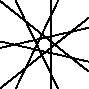
\includegraphics[height=1.5cm]{labsseptic1.pdf}
        &
        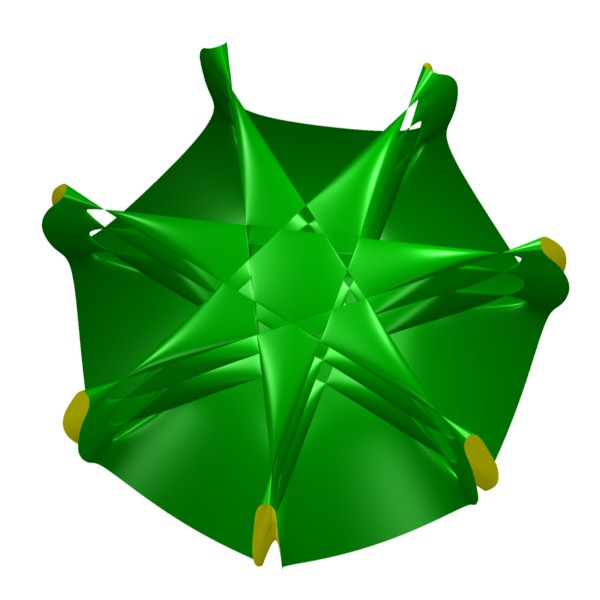
\includegraphics[height=1.5cm]{septic_7eck_von_oben}
      \end{tabular}
    \end{center}
    \vspace*{-0.3em}   
   Esta variante da constru\c c\~ao de Chmutov \'e da autoria de Duco van Straten.
\end{surferPage}
